%%%%%%%%%%%%%%%%%%%%%%%%%%%%%%%%%%%%%%%%%
% Beamer Presentation
% LaTeX Template
% Version 1.0 (10/11/12)
%
% This template has been downloaded from:
% http://www.LaTeXTemplates.com
%
% License:
% CC BY-NC-SA 3.0 (http://creativecommons.org/licenses/by-nc-sa/3.0/)
%
%%%%%%%%%%%%%%%%%%%%%%%%%%%%%%%%%%%%%%%%%

%----------------------------------------------------------------------------------------
%	PACKAGES AND THEMES
%----------------------------------------------------------------------------------------

\documentclass{beamer}

\mode<presentation> {

% The Beamer class comes with a number of default slide themes
% which change the colors and layouts of slides. Below this is a list
% of all the themes, uncomment each in turn to see what they look like.

%\usetheme{default}
%\usetheme{AnnArbor}
%\usetheme{Antibes}
%\usetheme{Bergen}
%\usetheme{Berkeley}
%\usetheme{Berlin}
%\usetheme{Boadilla}
%\usetheme{CambridgeUS}
%\usetheme{Copenhagen}
%\usetheme{Darmstadt}
\usetheme{Dresden}
%\usetheme{Frankfurt}
%\usetheme{Goettingen}
%\usetheme{Hannover}
%\usetheme{Ilmenau}
%\usetheme{JuanLesPins}
%\usetheme{Luebeck}
%\usetheme{Madrid}
%\usetheme{Malmoe}
%\usetheme{Marburg}
%\usetheme{Montpellier}
%\usetheme{PaloAlto}
%\usetheme{Pittsburgh}
%\usetheme{Rochester}
%\usetheme{Singapore}
%\usetheme{Szeged}
%\usetheme{Warsaw}

% As well as themes, the Beamer class has a number of color themes
% for any slide theme. Uncomment each of these in turn to see how it
% changes the colors of your current slide theme.

%\usecolortheme{albatross}
%\usecolortheme{beaver}
%\usecolortheme{beetle}
%\usecolortheme{crane}
%\usecolortheme{dolphin}
%\usecolortheme{dove}
%\usecolortheme{fly}
%\usecolortheme{lily}
%\usecolortheme{orchid}
%\usecolortheme{rose}
%\usecolortheme{seagull}
%\usecolortheme{seahorse}
%\usecolortheme{whale}
%\usecolortheme{wolverine}

%\setbeamertemplate{footline} % To remove the footer line in all slides uncomment this line
%\setbeamertemplate{footline}[page number] % To replace the footer line in all slides with a simple slide count uncomment this line

%\setbeamertemplate{navigation symbols}{} % To remove the navigation symbols from the bottom of all slides uncomment this line
}

\usepackage{graphicx} % Allows including images
\usepackage{booktabs} % Allows the use of \toprule, \midrule and \bottomrule in tables
\usepackage{wrapfig}
\usepackage{multimedia}

%----------------------------------------------------------------------------------------
%	TITLE PAGE
%----------------------------------------------------------------------------------------

\title[Design Phase]{Obstacle Avoidance and Goal Detection Robot using RPi and LRF.} % The short title appears at the bottom of every slide, the full title is only on the title page

\author{Atabak Hafeez \and
Maria Ficiu \and
Rubin Deliallisi \and
Siddharth Shukla} % Your name
\institute[Jacobs University Bremen] % Your institution as it will appear on the bottom of every slide, may be shorthand to save space
{
Jacobs University Bremen \\ % Your institution for the title page
\medskip
%\textit{john@smith.com} % Your email address
}
\date{\today} % Date, can be changed to a custom date

\begin{document}

\begin{frame}
\titlepage % Print the title page as the first slide
\end{frame}

\begin{frame}
\frametitle{Overview} % Table of contents slide, comment this block out to remove it
\tableofcontents % Throughout your presentation, if you choose to use \section{} and \subsection{} commands, these will automatically be printed on this slide as an overview of your presentation
\end{frame}


%----------------------------------------------------------------------------------------
%	PRESENTATION SLIDES
%----------------------------------------------------------------------------------------

%------------------------------------------------
\section{Rewind}
%------------------------------------------------

\subsection{Revisiting the Goals}
\begin{frame}
\frametitle{Goal}
\begin{quote}
Develop a robot using ROS that can navigate a maze based on the input from a laser range finder. 
\end{quote}
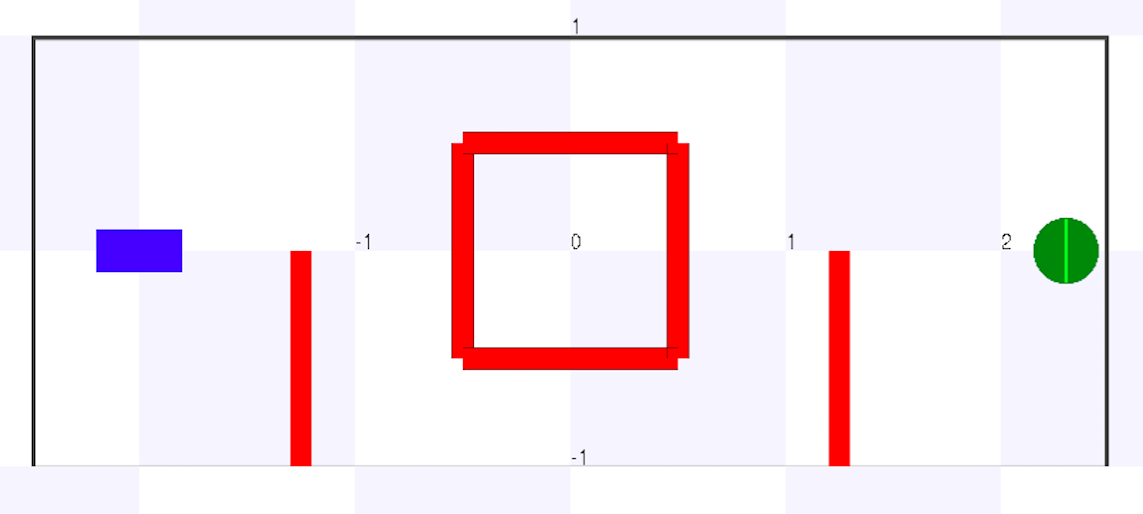
\includegraphics[scale=0.25]{assets/images/Visualization.png} 
\end{frame}

\subsection{Strategy}

\begin{frame}
\frametitle{Hough Transform}
\begin{wrapfigure}[10]{l}[0pt]{4cm}
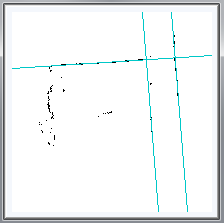
\includegraphics[scale=0.5]{assets/images/HoughTransform.png} 
\end{wrapfigure}
Detect imperfect instances of
\begin{itemize}
\item outer walls and obstacles, and
\item (semi) circles (i.e. goals)
\item OpenCV HoughLines and HoughCircle
\item Careful tuning of params for detecting real cases and avoiding false positives
\end{itemize}
\end{frame}

%\begin{frame}
%\frametitle{Bug Algorithms}
%\begin{wrapfigure}[10]{l}[0pt]{4cm}
%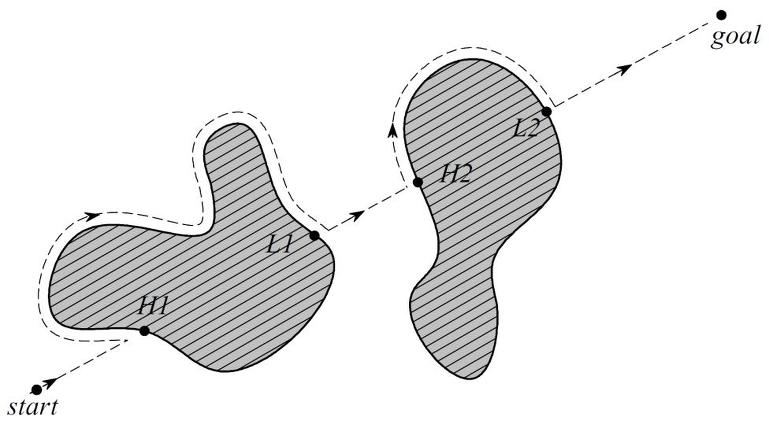
\includegraphics[scale=0.6]{assets/images/BugAlgorithms.jpg}
%\end{wrapfigure}
%(Modified) Bug algorithm for
%\begin{itemize}
%\item lack of encoder data, and
%\item Greedy problem solving
%\end{itemize}
%\end{frame}

\begin{frame}
\frametitle{Wall Following}
\begin{itemize}
\item Primary and Secondary security distances to avoid walls
\item Wall Follow distance used to stay close to wall with in place turns
\item Wall to be followed determined automatically
\item Upon Circle Detection, hit if spatial limits allow else follow wall
\end{itemize}
\end{frame}


\begin{frame}
\frametitle{Wall Following (Special cases)}
\begin{itemize}
\item Robot gets reset if it can't see a wall (too far) after consecutive in place turns.
\item Move towards the wall with a certain rotation in case the robot gets stuck in consecutive turn loop.
\item Set a threshold for the difference of wall vs obstacle turns in case robot gets stuck in a maze loop. 
\item Reset the robot state if beyond threshold count.
\end{itemize}
\end{frame}


%------------------------------------------------
\section{Software Development}
%------------------------------------------------
\subsection{Design Patterns}
\begin{frame}
\frametitle{Design Patterns}
\begin{itemize}
\item Singleton (i.e. Only one instance of a given class)
\item Publish-Subscribe (i.e. ROS nodes and topics)
\item Mediator (Encapsulating communication between objects. Abandoned eventually in favour of Pub/Sub)
\end{itemize}
\end{frame}

\begin{frame}
\frametitle{DevOps}
\begin{itemize}
\item Git (using Github for remote)
\item Divide tasks into issues
\item Branching Model
\begin{itemize}
\item Separate branch for each feature
\item Merge to develop after completion of issue
\item Rebase to develop at sprint end
\end{itemize}
\item Pre commit hooks for code style guideline compliance (only linting)
\end{itemize}
\end{frame}


\subsection{Workflow}
\begin{frame}
\frametitle{Stay Agile! Stay Alive!}
\begin{itemize}
\item Biweekly code sprints
\item Weekly review and retrospective
\item Coordinated Pair programming sessions
\end{itemize}
\end{frame}

\begin{frame}
\frametitle{Testing}
\begin{itemize}
\item Test Friendly Design Decisions
\begin{itemize}
\item Requires ROS parameters to initialize
\item Parameter loading through config files
\end{itemize}
\item Test Driven Development (TDD)
\begin{itemize}
\item Wrote tests before code
\item Helped clearly plan out program functionality
\item Reduced debug time drastically
\end{itemize}
\item Focused on different domains:
\begin{itemize}
\item Unit Testing (Google Tests and ROS tests)
\item System Testing (ROS tests)
\item Stress Testing  (ROS tests)
\end{itemize}
\end{itemize}
\end{frame}

%-----------------------
\section{Results}
%-----------------------

\subsection{Simulation}

\begin{frame}
\frametitle{Simulation}
\begin{itemize}
\item Great for rapid prototyping
\item Helpful for TDD (automated test suites)
\item Easy to benchmark
\end{itemize}
\end{frame}

\begin{frame}{Simulation (goal)}
\begin{figure}[h!]
\centering    
\movie[label=show3,width=1.0\textwidth,poster
       ,autostart,showcontrols,loop] 
  {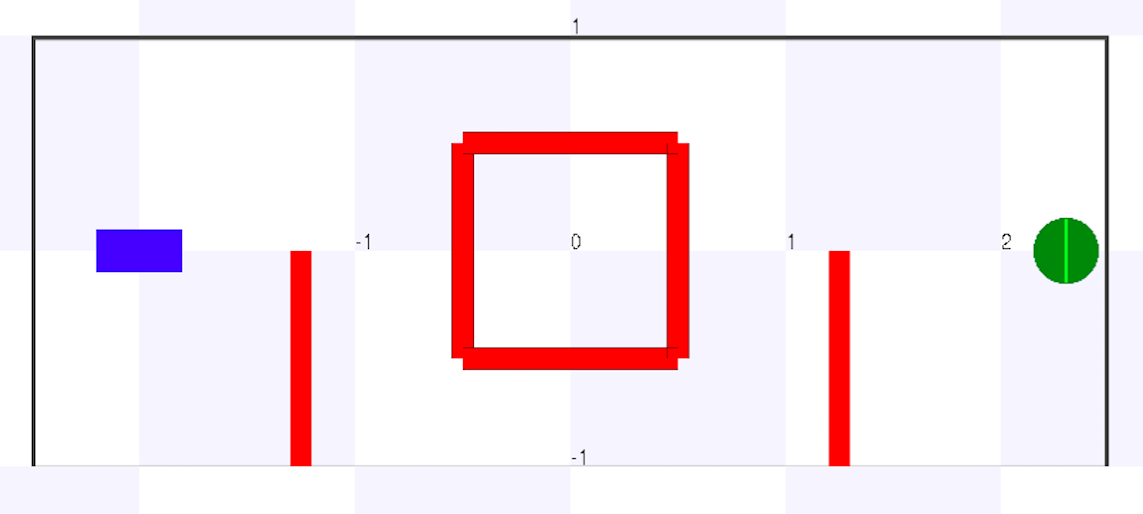
\includegraphics[width=1.0\textwidth]{media1.png}}{media1.mp4}
  \caption{Simulation on different levels}
 \end{figure} 
  \end{frame}
  
\begin{frame}{Simulation (loop detection)}
\begin{figure}[h!]
\centering    
\movie[label=show3,width=1.0\textwidth,poster
       ,autostart,showcontrols,loop] 
  {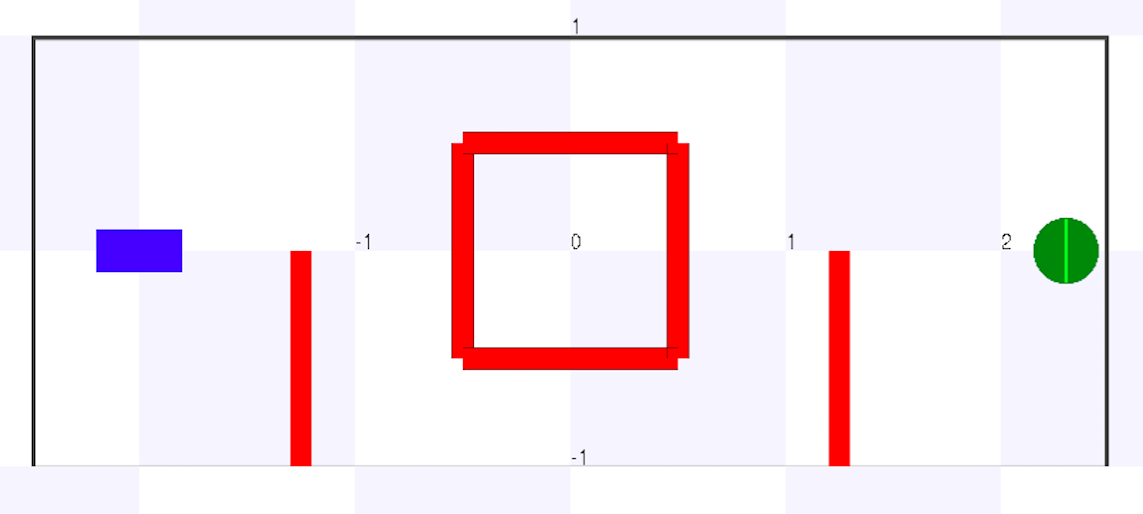
\includegraphics[width=1.0\textwidth]{media1.png}}{media2.mp4}
  \caption{Simulation on different levels}
 \end{figure} 
  \end{frame}

\subsection{Real World}

\begin{frame}
\frametitle{Real World}
\begin{itemize}
\item Unsuspecting differences between Simulation and Real World
\item Everything more prone to errors and Data more noisy
\item Increased Linear and Angular velocities for Real world
\item Decreased wall follow distance because of data delay
\item Adjust circle hit mode to do adaptive refinement of movement direction
\end{itemize}
\end{frame}

%------------------------------------------------
\section{References}
%------------------------------------------------
\begin{frame}
\frametitle{References}
\footnotesize{
\begin{thebibliography}{99} % Beamer does not support BibTeX so references must be inserted manually as below
\bibitem[MARS, 2016]{p1} Atabak Hafeez, Maria Ficiu, Rubin Deliallisi, Siddharth Shukla (2016)
\newblock Obstacle Avoidance and Goal Detection Robot
\newblock \emph{Jacobs University Bremen}.

\bibitem[Misha, 2004]{p1} Michael Misha Kazhdan(2004)
\newblock Seminar on Shape Analysis and Retrieval
\newblock \emph{Department of Computer Science,
Johns Hopkins University, Baltimore, MD}.

\bibitem[Choset]{p1} Howie Choset
\newblock Robotic Motion Planning: Bug Algorithms
\newblock \emph{The Robotics Institute,
Carnegie Mellon University, Pittsburgh, PA}.

\end{thebibliography}
}
\end{frame}

%----------------------------------------------------------------------------------------
\end{document} 
